\documentclass[../main.tex]{subfiles}


\begin{document}
Zum Abschluss der Arbeit sollten die Implementierungen des CNN untereinander, sowie mit dem Beispiel auf Basis von Tensorflow, hinsichtlich ihrer Schnelligkeit (die Qualität bzw. Verwendbarkeit der Ergebnisse wird für die einzelnen Implementierungen getrennt betrachtet) verglichen werden. Um vergleichbare Ergebnisse zu erhalten, werden auf jedem Testsystem mehrere Implementierungen getestet. Für die Durchführung der Tests kommen zwei Rechner zum Einsatz: 
\begin{description}
\item[it-phi] Ein Zugang zu diesem Server wurde den Studenten für diese Arbeit freundlicherweise von der DHBW Stuttgart zur Verfügung gestellt: Er ist mit zwei Server-CPUs (Intel Xeon E5-2650L) und einem Coprozessor (Intel Xeon Phi) ausgestattet. Beim Xeon Phi handelt es sich um eine PCIe-Erweiterungskarte, auf der eine spezielle CPU mit 60 Kernen und einer Taktrate von 1\,GHz, sowie ein DDR5-Arbeitsspeicher mit einer Größe von 8\,GB verbaut sind. 
\item[Zweiter Testrechner] Zum Testen der Implementierung für CUDA wird ein weiterer Testrechner benötigt. Dieser besitzt eine Intel-CPU (Core I7-7700HQ) sowie eine NVidia GTX1070. 
\end{description}
Alle Implementierungen werden für die Programmtests derart angepasst, dass sie Trainingsdurchläfe und Evaluierungen für eine bestimmte Anzahl von Bildern durchführen. Idealerweise sollten Trainings- und Testläufe für je 1000, 10000 und 20000 Bilder durchgeführt werden. Tatsächlich werden nicht für jede Implementierung alle Werte bestimmt. Die serielle Implementierung wird mit je 100, 500 und 1000 Bildern getestet. Größere Datenmengen können von der seriellen Implementierung nicht in akzeptabler Zeit verarbeitet werden. 

Alle getesteten Implementierungen basieren auf dem gleichen Netzaufbau. Als erstes gibt es einen Convolutional Layer mit einem Faltungskern mit 5*5 Elementen und 32 Feature Maps am Ende des Layers. Anschließend folgt ein Max Pooling Layer, der das Maximum aus 2*2 Quadraten aussucht. Anschließend folgt ein weiterer Convolutional Layer mit der selben Größe der Faltungskerne und diesmal 64 Feature Maps, sowie ein zweiter Max Pooling Layer. Am Ende folgen noch zwei Fully Connected Layer mit einer Größe von einmal 1024 Elementen und einmal 10 Elementen.

Zum Messen der Ausführungsdauer wurde das Linuxtool \texttt{time} verwendet. Dieses kann vor einem beliebigen Befehl in der Shell geschrieben werden. Ist der mitgegebene Befehl ausgeführt, zeigt \texttt{time} die vergangene zeit seit Beginn der Ausführung an. Dabei wird unterschieden in die tatsächlich verstrichene Zeit, die Zeit im User-Modus und die Zeit im Kernel-Modus.

Auf dem Server it-phi werden die Implementierungen für x86-CPUs, für die Tensorflow-Vorlage und für den Intel Xeon Phi getestet. 

Das Messen der Ausführungszeit für die Implementierung auf einer x86 CPU auf dem Server it-phi ergab dabei folgende Werte:\par

\begin{tabular}{|c|c||c|c|}
	\hline
	\multicolumn{2}{|c||}{1000 Durchläufe} & \multicolumn{2}{c|}{20000 Durchläufe} \\ \hline
	real & 1m 53,461s & real & 36m 57,646s\\ 
	\hline
	user & 44m 55,92s & user & 1082m 4,68s \\ 
	\hline
	sys & 0m 2,30s & sys & 0m 32,752s\\ 
	\hline
\end{tabular}

Zu erkennen ist, dass die Zeit im User-Mode zirka um den Faktor 30 Größer ist, als die tatsächliche Ausführungszeit.
Dies liegt am Multithreading des Programms. Wird während der Ausführung mit dem Befehl \texttt{top} die Auslastung des Prozessors angezeigt ist zu sehen, dass die Auslastung der CPU bei 2915\% liegt. Dem Server stehen insgesamt 32 CPU-Threads zur Verfügung, \texttt{top} rechnet dies auf einen CPU-Kern und so ist es möglich, mehr als 100\% Prozessorauslastung angezeigt zu bekommen.
\begin{figure}[!htbp]
	\centering
	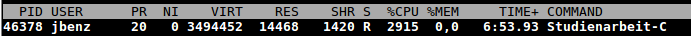
\includegraphics[width=0.7\textwidth]{../images/Benz/screenshot_top.png} %Screenshot top
	\caption{Eintrag mit Prozessorauslastung der x86-Implementierung} 
\end{figure}

Bei der Ausführung der beiden anderen Implementierungen ergeben sich kürzere Laufzeiten für gleiche Datenmengen. Die nachfolgenden Diagramme zeigen, dass sich die Laufzeiten annähernd linear zur verarbeiteten Datenmenge verhalten. Ist der genaue Zusammenhang zwischen Datenmenge und Laufzeit bekannt, lassen sich daraus Schlüsse über die Dauer der Initialisierung und die durchschnittliche Verarbeitungszeit pro Bild ziehen. 

Wie in den Diagrammen in Abbildung \ref{pics:diagrams_speedtest} abzulesen ist, benötigt die Implementierung für den Xeon Phi im Gegensatz zur Vorlage eine wesentlich größere Laufzeit zur Initialisierung des Programms. Allerdings ist die durchschnittliche Laufzeit zur Bearbeitung eines einzelnen Bildes wesentlich geringer. Beim Testdurchgang mit 20000 Trainingsbildern ist die gesamte Laufzeit der Implementierung für den Xeon Phi bereits geringer als die von der Vorlage benötigte Zeit. Die für eine einzelne Evaluierung benötigte Laufzeit ist wesentlich geringer als die Laufzeit eines Trainingsdurchgangs. In den Diagrammen ist dies anhand der deutlich langsamer steigenden Linien zu erkennen. Auch der Unterschied zwischen den Implementierungen fällt beim evaluieren wesentlich geringer aus. Daraus lässt sich folgern, dass die Implementierung für den Xeon Phi bei großen Mengen von Trainingsdaten auf diesem Server tatsächlich schneller arbeitet als Tensorflow. Der Grund dafür liegt allerdings nicht darin, dass die Implementierung für den Xeon Phi allgemein effizienter arbeiten würde. Der tatsächliche Grund ist, dass Tensorflow nicht zur Nutzung eines Coprozessors ausgelegt ist und den Xeon Phi nicht verwenden kann. 

\begin{figure}
	\begin{subfigure}{0.49\textwidth}
		\centering
		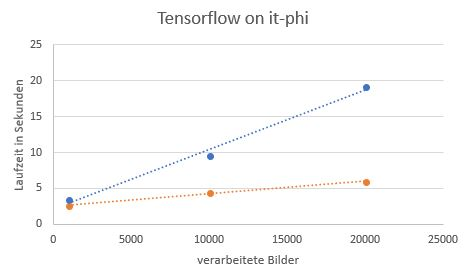
\includegraphics[width=\linewidth]{../images/Schmidt/bm_tf_phi.jpg}
	\end{subfigure}%
	\begin{subfigure}{0.49\textwidth}
		\centering
		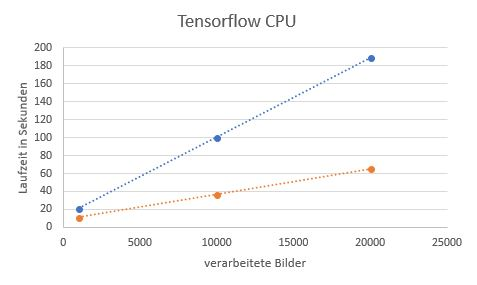
\includegraphics[width=\linewidth]{../images/Schmidt/bm_tf_std.jpg}
	\end{subfigure}

	\begin{subfigure}{0.49\textwidth}
		\centering
		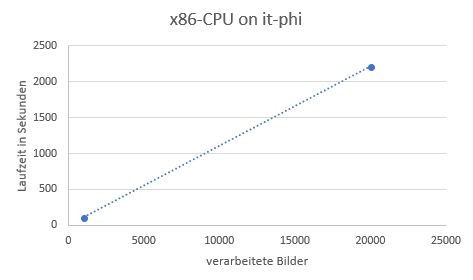
\includegraphics[width=\linewidth]{../images/Schmidt/bm_x86_phi.jpg}
	\end{subfigure}%
	\begin{subfigure}{0.49\textwidth}
		\centering
		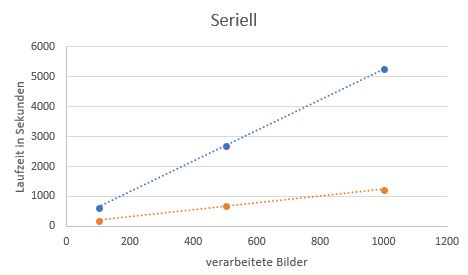
\includegraphics[width=\linewidth]{../images/Schmidt/bm_serial_std.jpg}
	\end{subfigure}

	\begin{subfigure}{0.49\textwidth}
		\centering
		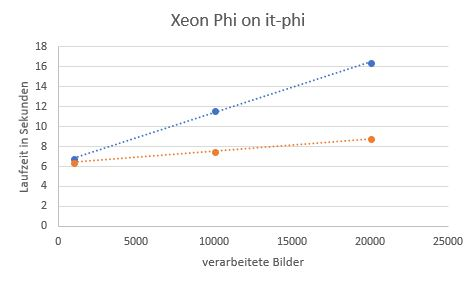
\includegraphics[width=\linewidth]{../images/Schmidt/bm_phi_phi.jpg}
	\end{subfigure}%
	\begin{subfigure}{0.49\textwidth}
		\centering
		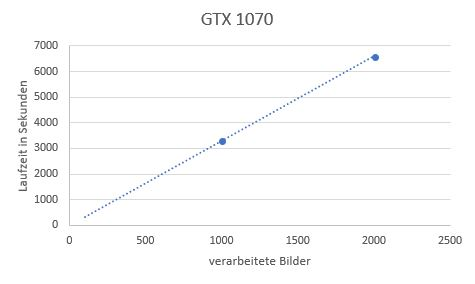
\includegraphics[width=\linewidth]{../images/Schmidt/bm_gtx_std.jpg}
	\end{subfigure}%
	\caption{Ergebnisse auf dem zweiten Testrechner}
	\label{pics:diagrams_speedtest} 
\end{figure}

Auf dem zweiten Testrechner werden die serielle Implementierung, die Implementierung zur Nutzung von GPUs mithilfe von CUDA und zu Vergleichszwecken die Tensorflow-Vorlage (ohne Nutzung der GPU) getestet. Abbildung \ref{pics:diagrams_speedtest} zeigt Diagramme zu den für diesen Rechner ermittelten Testergebnissen. Wie am Diagramm für Tensorflow zu erkennen ist, benötigt das Referenzskript auf diesem Rechner die zehnfache Laufzeit gegenüber der Server-CPU auf dem it-phi. Die Implementierungen dieses Testlaufs lassen sich nur bedingt miteinander vergleichen. Um die Programmtests in akzeptabler Zeit abschließen zu können, werden die serielle Implementierung, sowie die Implementierung zur Nutzung von GPUs mit kleineren Datenmengen getestet. Aus dem zugehörigen Diagramm lässt sich trotzdem gut ablesen, dass die serielle Implementierung das langsamste aller hier betrachteten Programme ist. Dies entspricht auch den Erwartungen; sie ist weder zur Nutzung von Parallelisierung, noch durch Vektorisierung optimiert. Obwohl der Implementierung für CUDA im Gegensatz zu Tensorflow in der Lage ist, Rechenoperationen auf eine Grafikkarte auszulagern, ist sie deutlich langsamer als die Referenzimplementierung. Der Grund für die lange Laufzeit des CUDA-Programms liegt vermutlich in der Auslagerung von Code, der bedingte Sprünge enthält. GPUs sind zwar prinzipiell zur Ausführung von verzweigtem Code fähig, allerdings läuft dieser sehr ineffizient. Auf die schlechte Eignung von GPUs für branch prediction wird bereits in Abschnitt \ref{sec:cuda_staerken} hingewiesen. Möglicherweise ergibt sich eine weitere Verlängerung der Laufzeit durch die Verwendung von \emph{dynamic parallelism} anstatt \emph{konkurrierender Streams}. Eine Vergleich dieser Parallelisierungsansätze ist allerdings nicht Teil der Arbeit und wurde in deren Verlauf auch nicht durchgeführt. 

Die Bewertung verschiedener Lösungsansätze hinsichtlich der Eignung für den konkreten Anwendungsfall stellt allgemein für alle in dieser Arbeit erstellten Programme die größte Herausforderung dar. Es ist davon auszugehen, dass alle erstellten Implementierungen hinsichtlich ihrer Effizienz weiter verbessert werden können. 

\end{document}